%% LyX 2.2.3 created this file.  For more info, see http://www.lyx.org/.
%% Do not edit unless you really know what you are doing.
\documentclass[oneside,english]{extbook}
\usepackage{lmodern}
\renewcommand{\sfdefault}{lmss}
\renewcommand{\ttdefault}{lmtt}
\usepackage[T1]{fontenc}
\usepackage[latin9]{inputenc}
\usepackage{geometry}
\geometry{verbose,tmargin=25mm,bmargin=25mm,lmargin=25mm,rmargin=25mm}
\pagestyle{plain}
\setcounter{secnumdepth}{3}
\setcounter{tocdepth}{3}
\setlength{\parindent}{0bp}
\usepackage{babel}
\usepackage{float}
\usepackage{graphicx}
\usepackage{setspace}
\onehalfspacing
\usepackage[unicode=true,pdfusetitle,
 bookmarks=true,bookmarksnumbered=false,bookmarksopen=false,
 breaklinks=false,pdfborder={0 0 1},backref=false,colorlinks=false]
 {hyperref}

\makeatletter
%%%%%%%%%%%%%%%%%%%%%%%%%%%%%% User specified LaTeX commands.
\usepackage{amssymb}
\usepackage{color}
\usepackage{listings}
\definecolor{hellgelb}{rgb}{1,1,0.85}
\definecolor{colKeys}{rgb}{0,0,1}
\definecolor{colIdentifier}{rgb}{0,0,0}
\definecolor{colComments}{rgb}{1,0,0}
\definecolor{colString}{rgb}{0,0.5,0}
\lstset{
      language=Matlab,
      float=hbp,
      basicstyle=\footnotesize\ttfamily,
      identifierstyle=\color{colIdentifier},
      keywordstyle=\color{colKeys},
      stringstyle=\color{colString},
      commentstyle=\itshape\color{colComments},
      columns=fixed,
      tabsize=4,
      frame=single,
      framerule=1pt,
      extendedchars=true,
      showspaces=false,
      showstringspaces=false,
      numbers=left,
      numberstyle=\tiny\ttfamily,
      numbersep=1em,
      breaklines=true,
      breakindent=10pt,
      backgroundcolor=\color{hellgelb},
      breakautoindent=true,
      captionpos=t,
      xleftmargin=1em,
      xrightmargin=\fboxsep
}
\usepackage{lscape}
\usepackage{amsmath}
\usepackage{mathtools}
\usepackage{pifont}
\usepackage{color}
\usepackage{accents}

\delimitershortfall=-1pt
\let\Right\right
\let\Left\left
\makeatletter
\def\right#1{\Right#1\@ifnextchar){\!\right}{}}
\def\left#1{\Left#1\@ifnextchar({\!\left}{}}
\makeatother

\makeatother

\begin{document}
\pagenumbering{gobble}

\begin{figure}[H]
\centering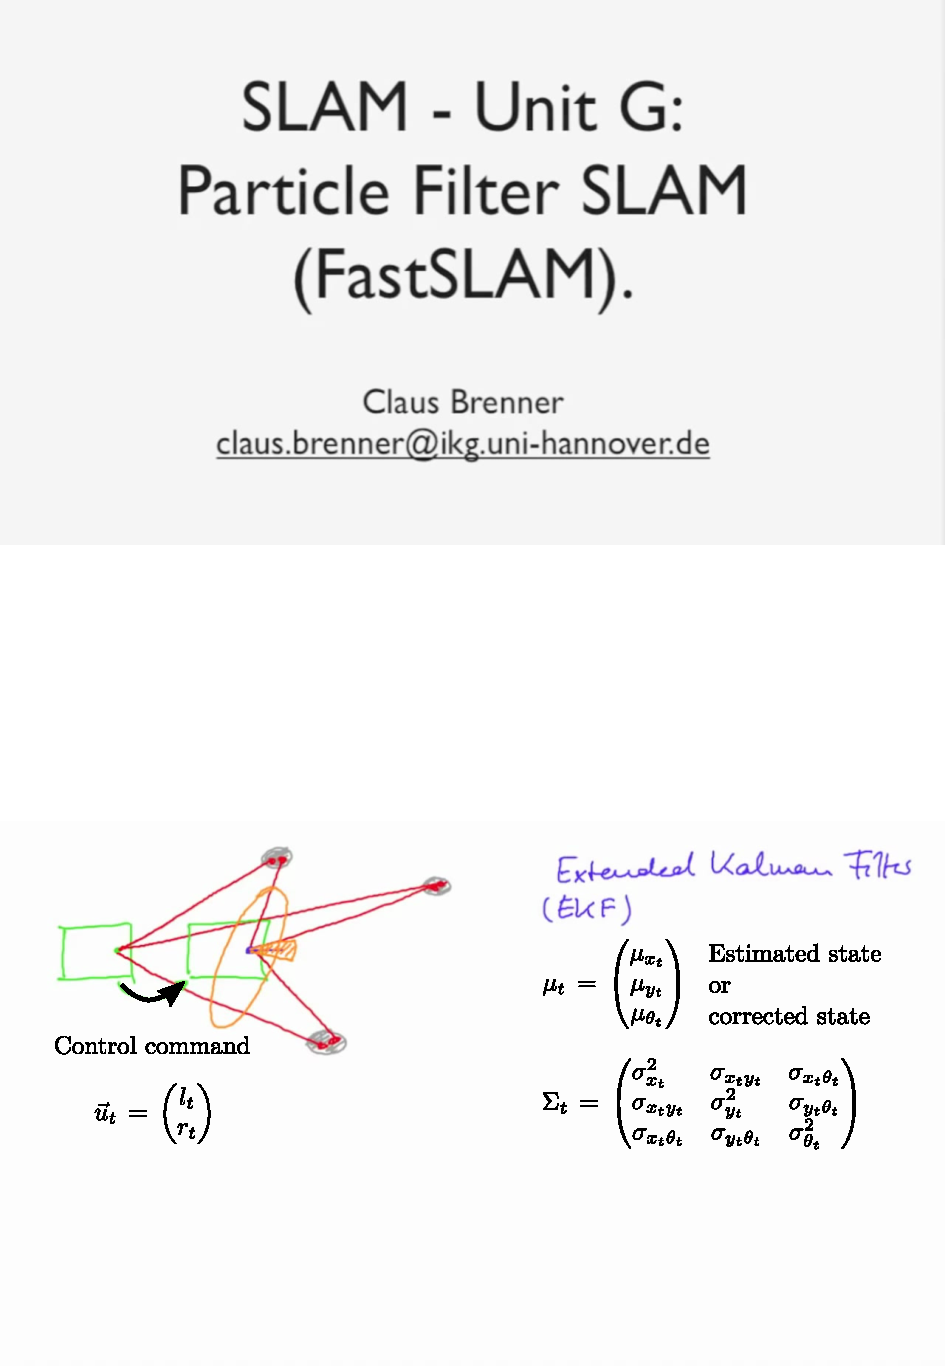
\includegraphics[scale=0.95]{../FIGURES/fig04}
\end{figure}

\begin{figure}[H]
\centering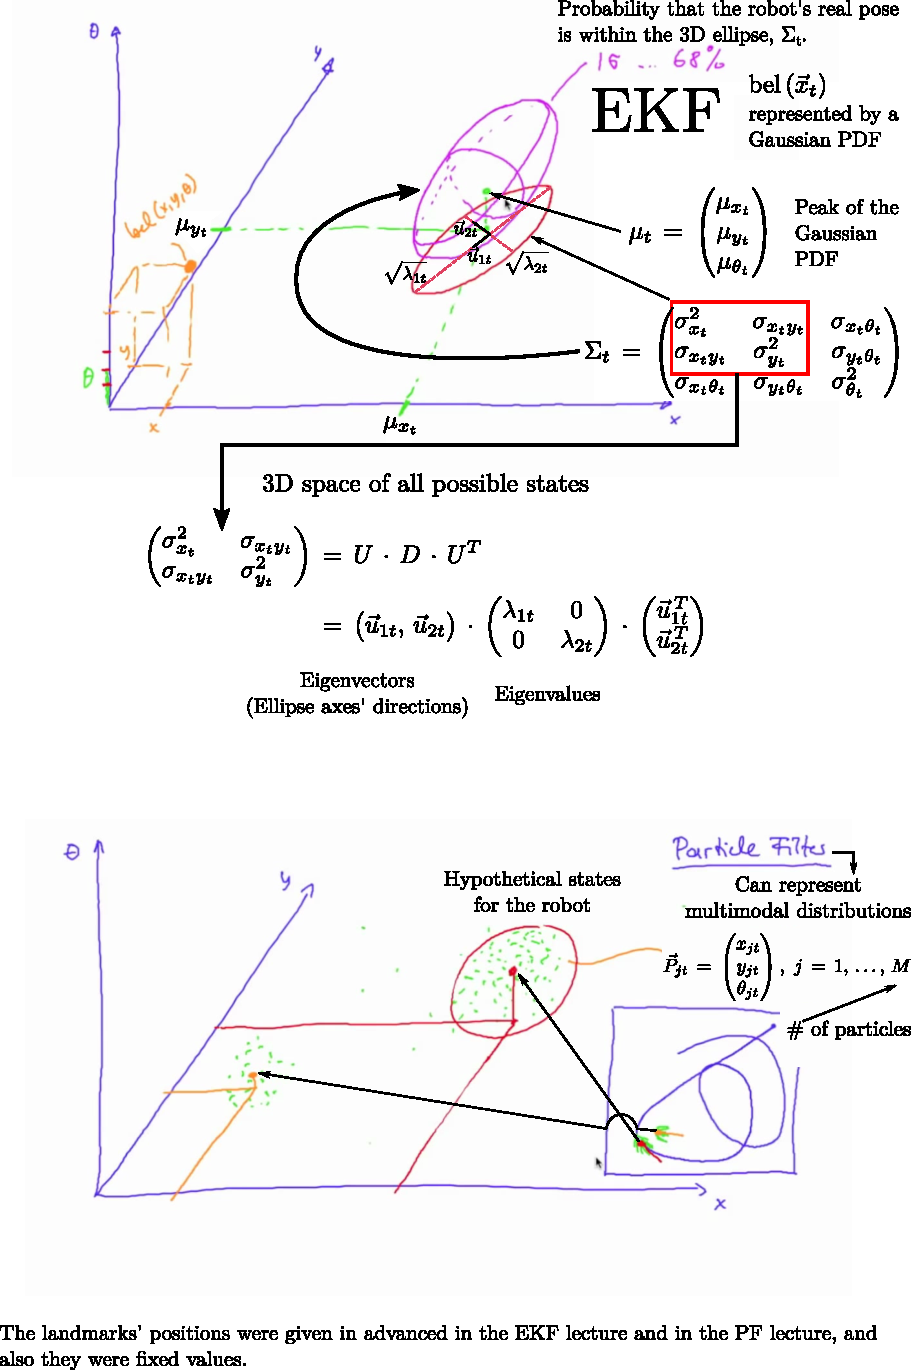
\includegraphics[scale=0.95]{../FIGURES/fig08}
\end{figure}

\begin{figure}[H]
\centering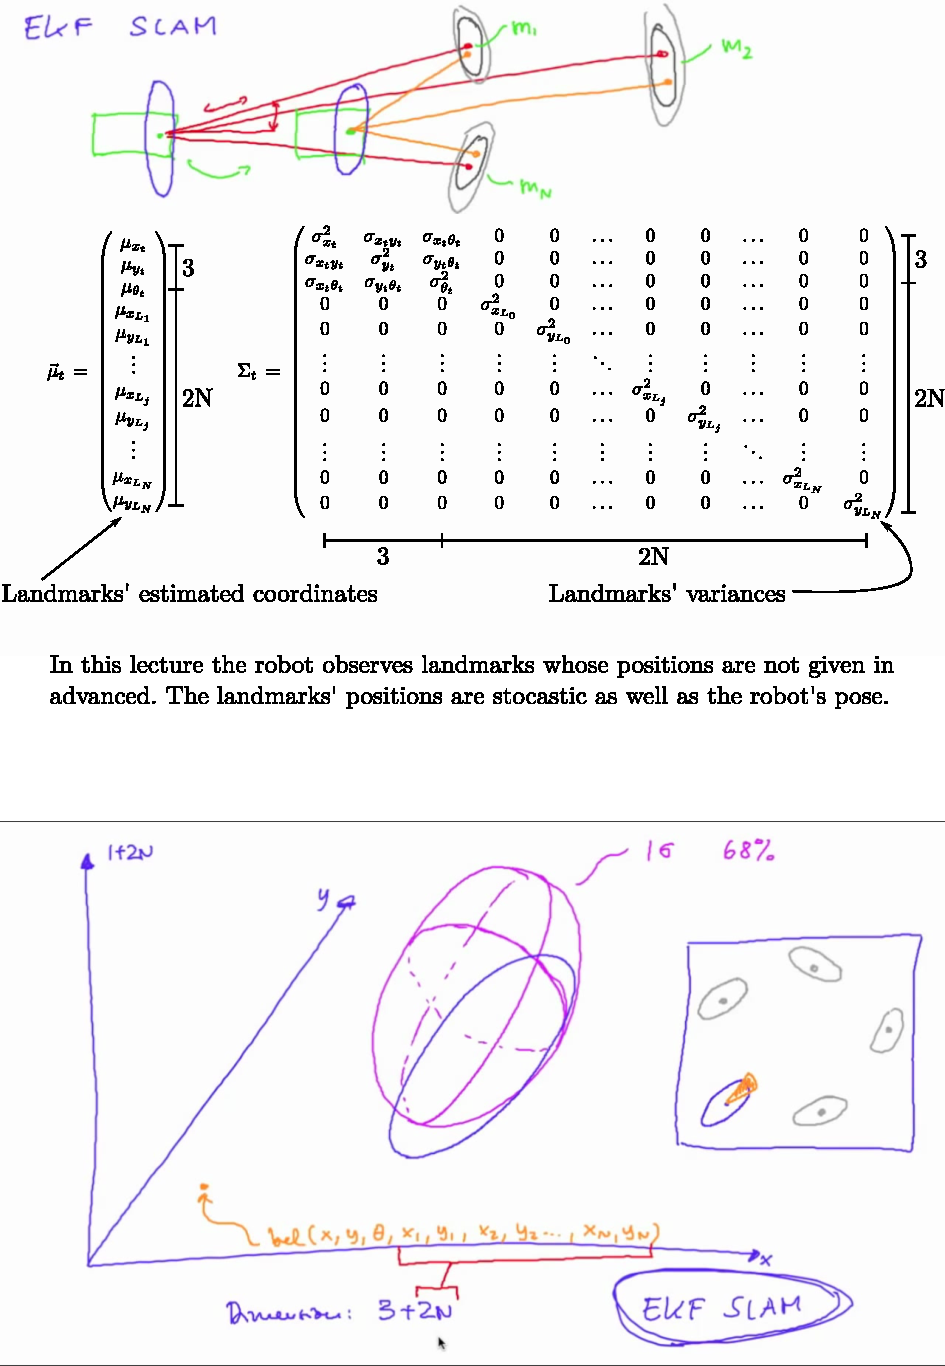
\includegraphics[scale=0.95]{../FIGURES/fig12}
\end{figure}

\begin{figure}[H]
\centering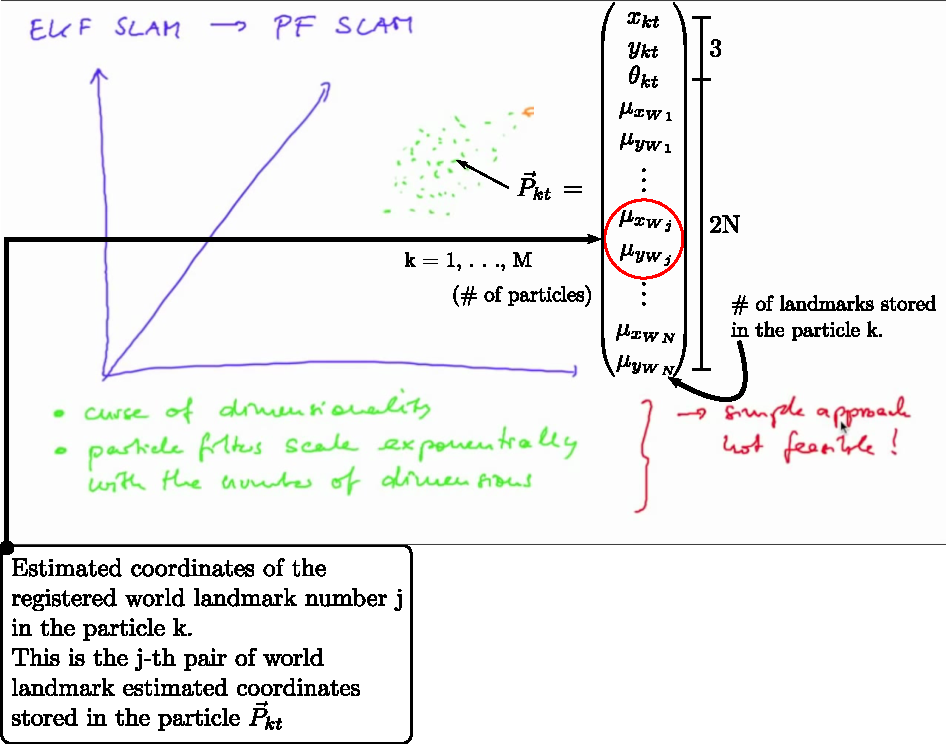
\includegraphics[scale=0.95]{../FIGURES/fig15}
\end{figure}

\textbf{Curse of dimensionality:}

The particle filter scales exponentially with the number of dimensions.
This means that if the dimension of the search space increase, the
number of particles that are necessary to represent the posterior
distribution scales exponentially. Therefore, this approach is unfeasible.

The new approach will be\textbf{the Rao-Blackwellized Particle Filter
(RBPF)}, where the posterior PDF is factorized as:

\begin{figure}[H]
\centering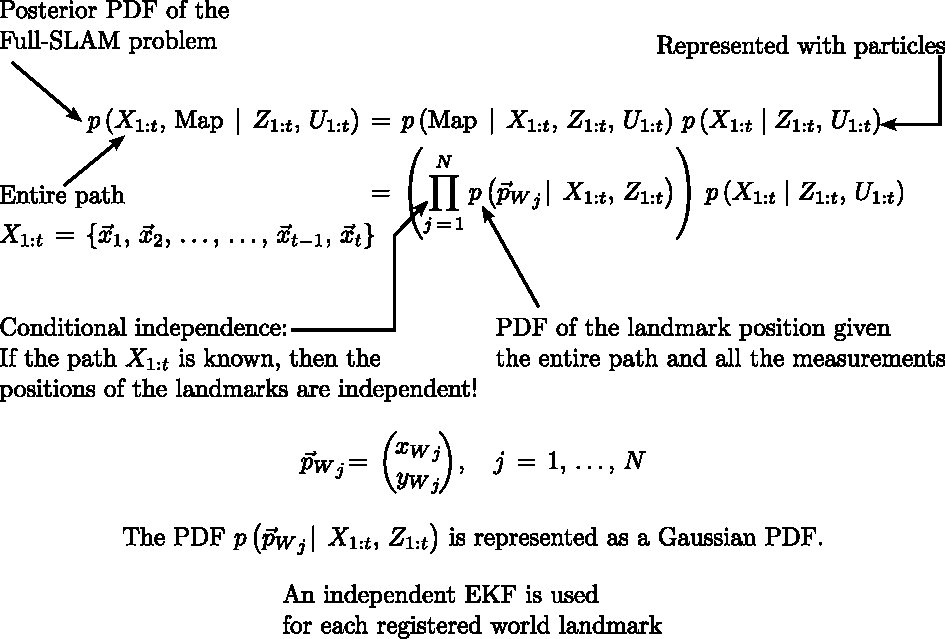
\includegraphics[scale=0.95]{../FIGURES/fig16}
\end{figure}

The term

\begin{align*}
{\vec{p}_W}_j\,=\,\begin{pmatrix}{x_W}_j\\ {y_W}_j\end{pmatrix}
\end{align*}

$j\,=\,1,\,\ldots,\,N$, represents the random coordinates of the
registered world landmark number$j$ within the state vector$\vec{x}_t$.

The term

\begin{align*}
\vec{\mu}_{L_j}\,=\,\begin{pmatrix}\mu_{{x_W}_j}\\\,\mu_{{y_W}_j}\end{pmatrix}
\end{align*}$j\,=\,1,\,\ldots,\,N$, represents the estimated coordinates of the
registered world landmark number$j$ within a specific particle,$\vec{P}_{kt}, ~ k\,=\,1,\,\ldots,\,M$.

The index where the estimated$x$ coordinate for the registered world
landmark$j$,$\mu_{{x_W}_j}$, is stored within a specific particle,$\vec{P}_{kt}$,
is\footnote{The same idea applies for the random the random coordinate${x_W}_j$
within the state vector$\vec{x}_t$}:

\[
i\,=\,3\,+\,2\,j\,-\,1
\]

The\textbf{Rao-Blackwellized Particle Filter (RBPF)} is given without
a proof!

Summarize: The PDF of the robot's pose is represented using a particle
filter. For each particle, the remaining part of the posterior PDF
is represented by an independent Gaussian PDF, which is the result
of an independent EKF.

\begin{figure}[H]
\centering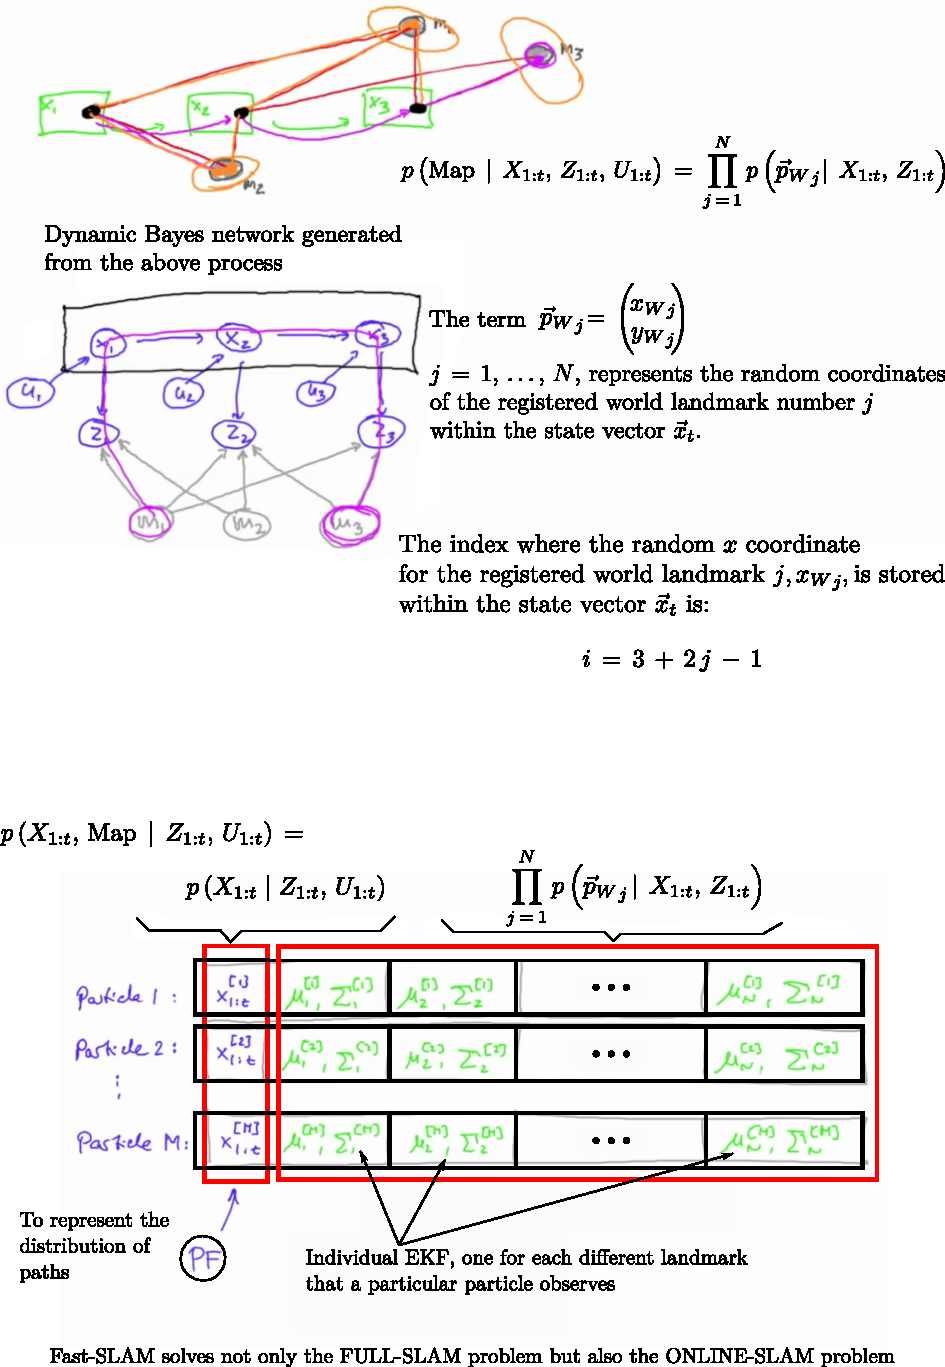
\includegraphics[scale=0.95]{../FIGURES/fig20}
\end{figure}

\begin{figure}[H]
\centering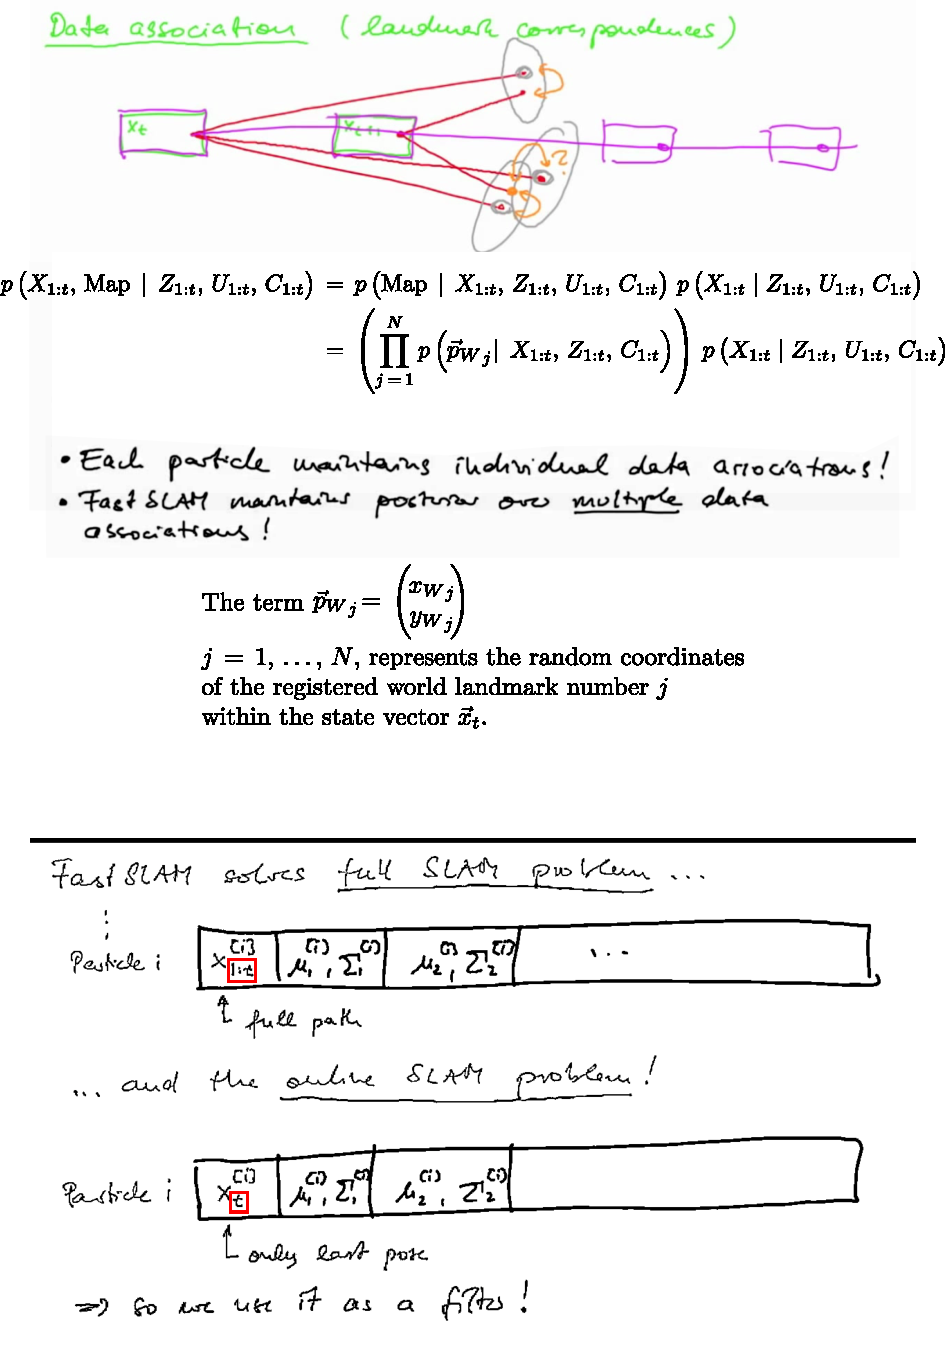
\includegraphics[scale=0.95]{../FIGURES/fig25}
\end{figure}

\begin{figure}[H]
\centering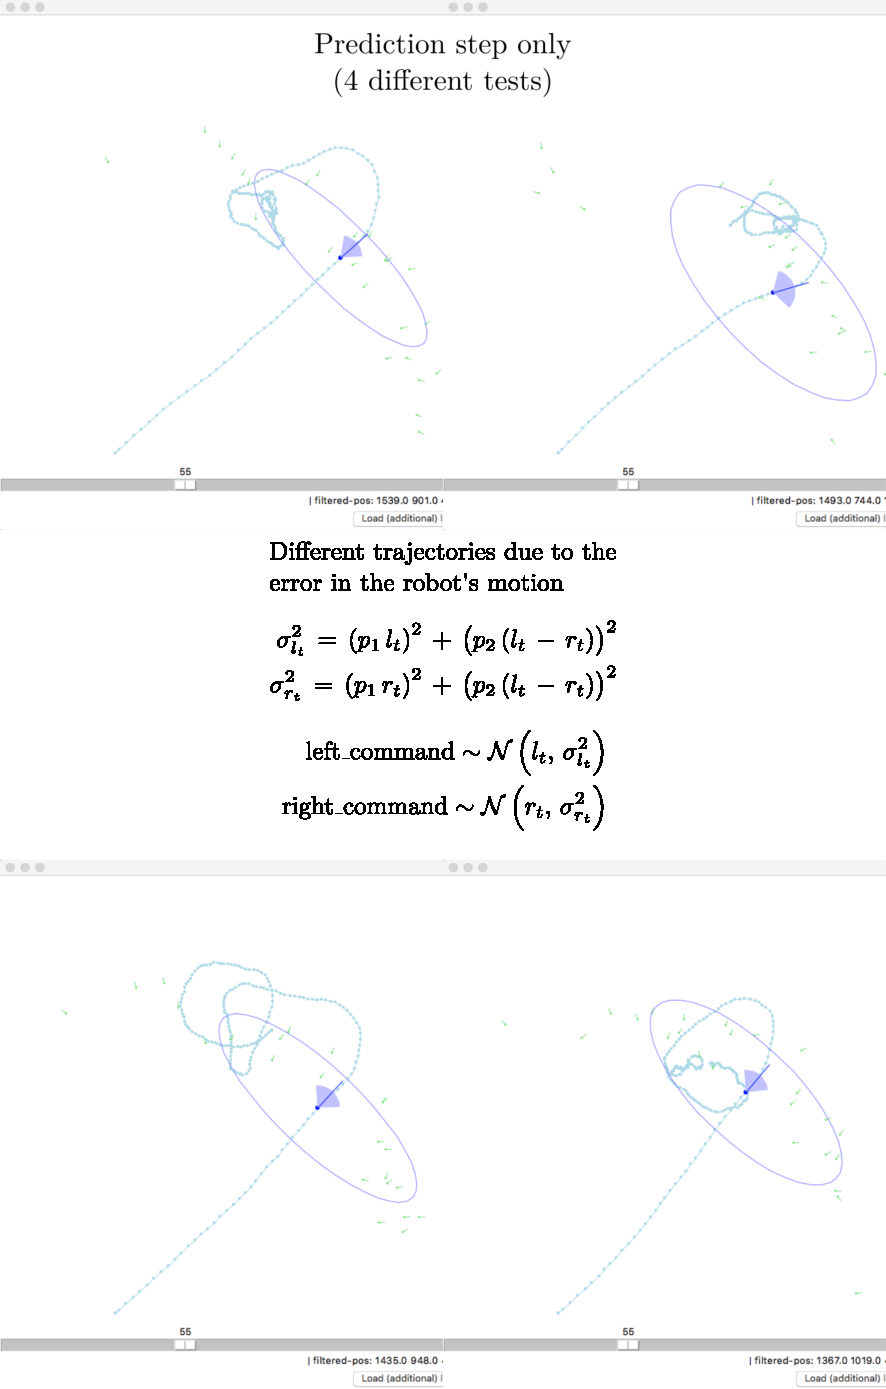
\includegraphics[scale=0.95]{../FIGURES/fig28}
\end{figure}

\begin{figure}[H]
\centering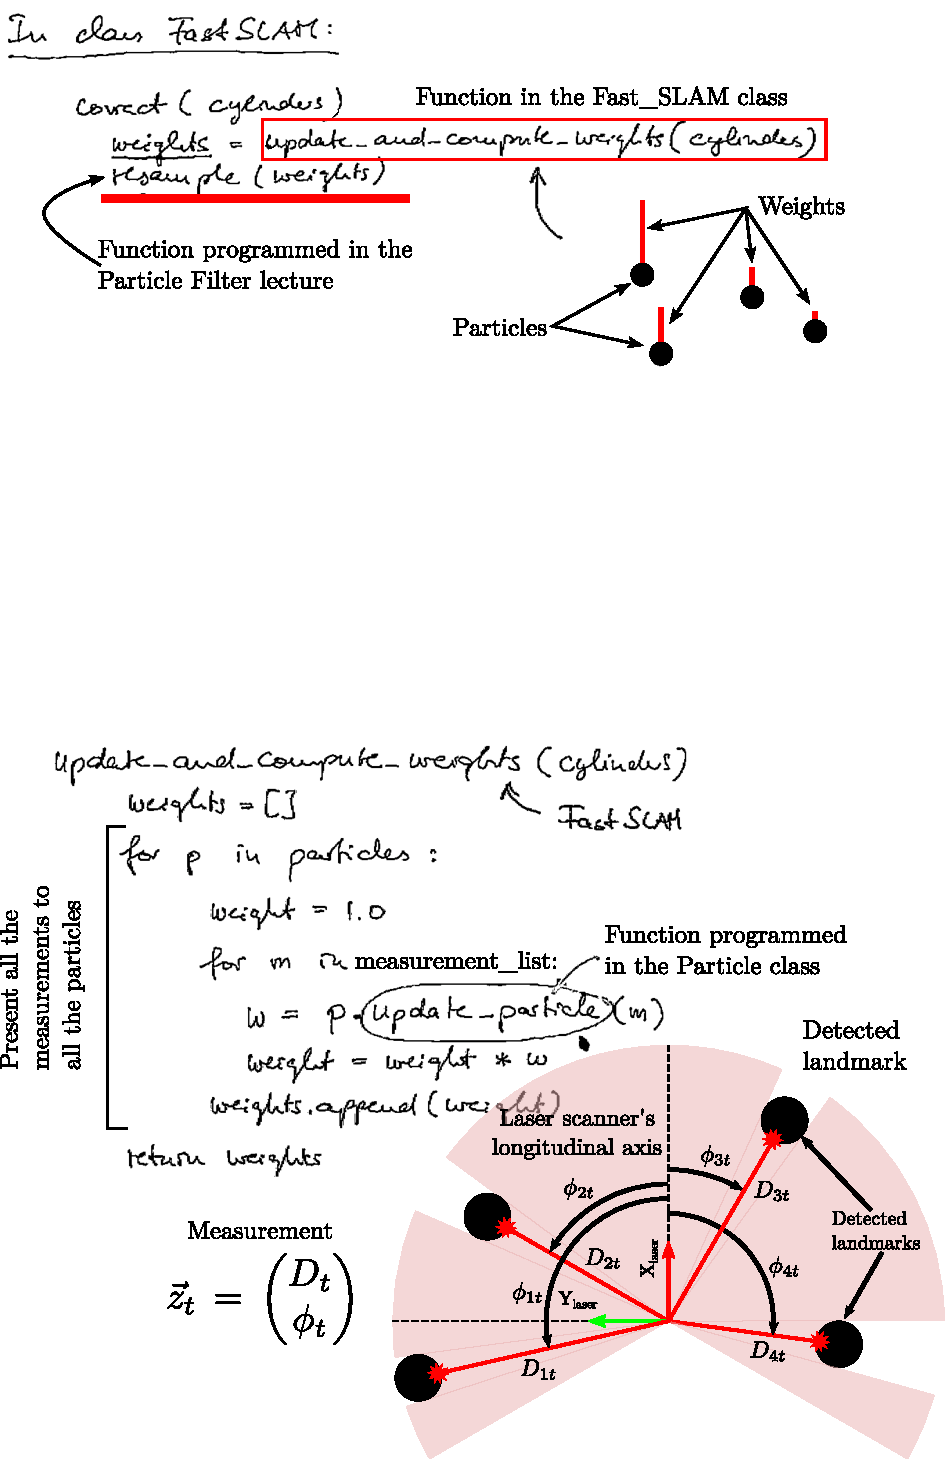
\includegraphics[scale=0.95]{../FIGURES/fig35}
\end{figure}

\begin{figure}[H]
\centering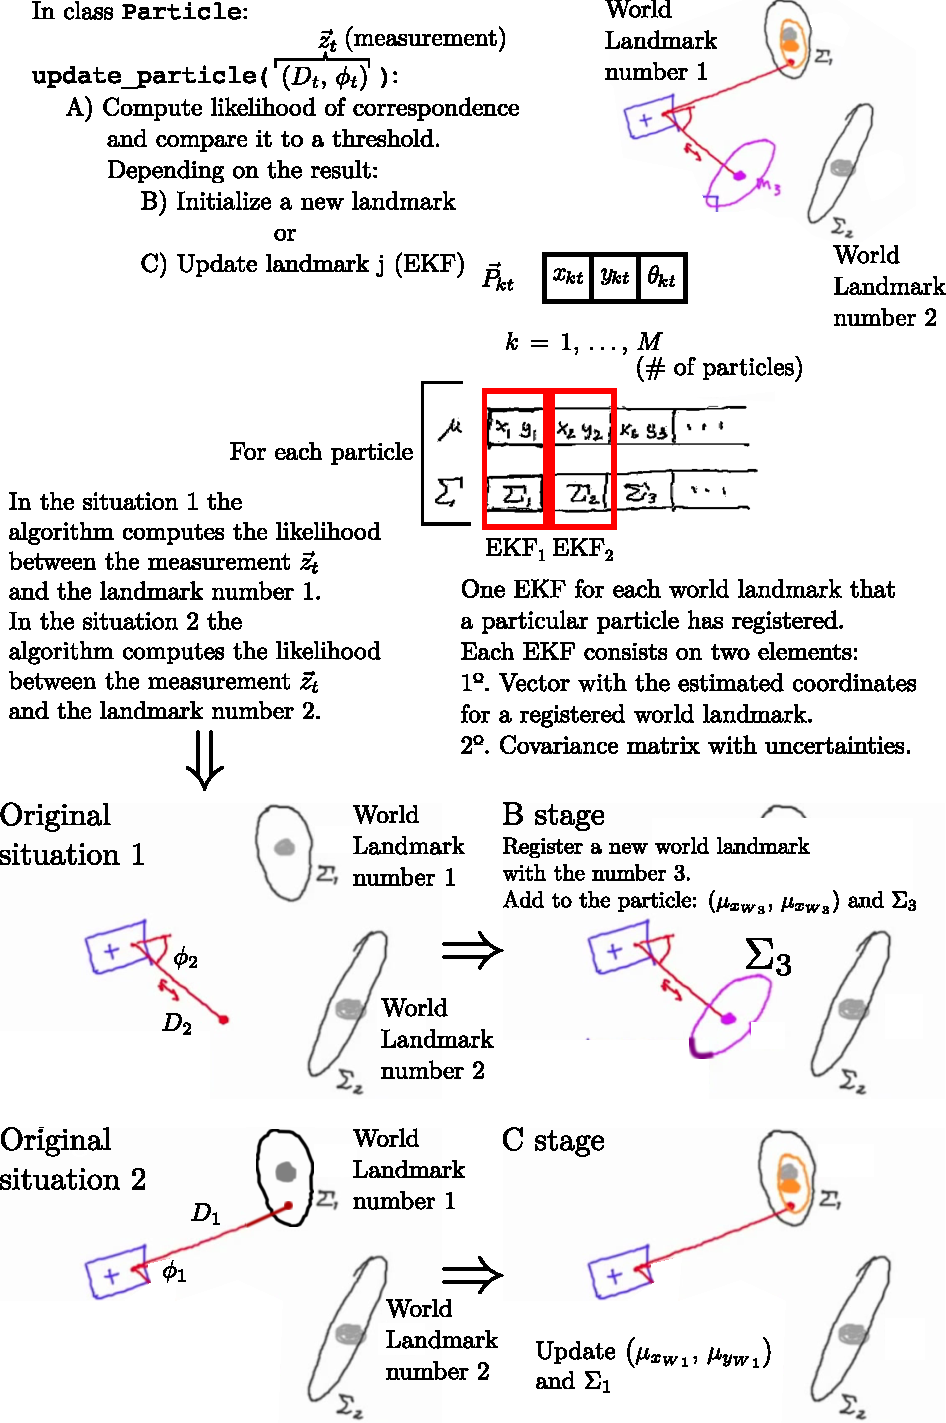
\includegraphics[scale=0.95]{../FIGURES/fig39}
\end{figure}

\begin{figure}[H]
\centering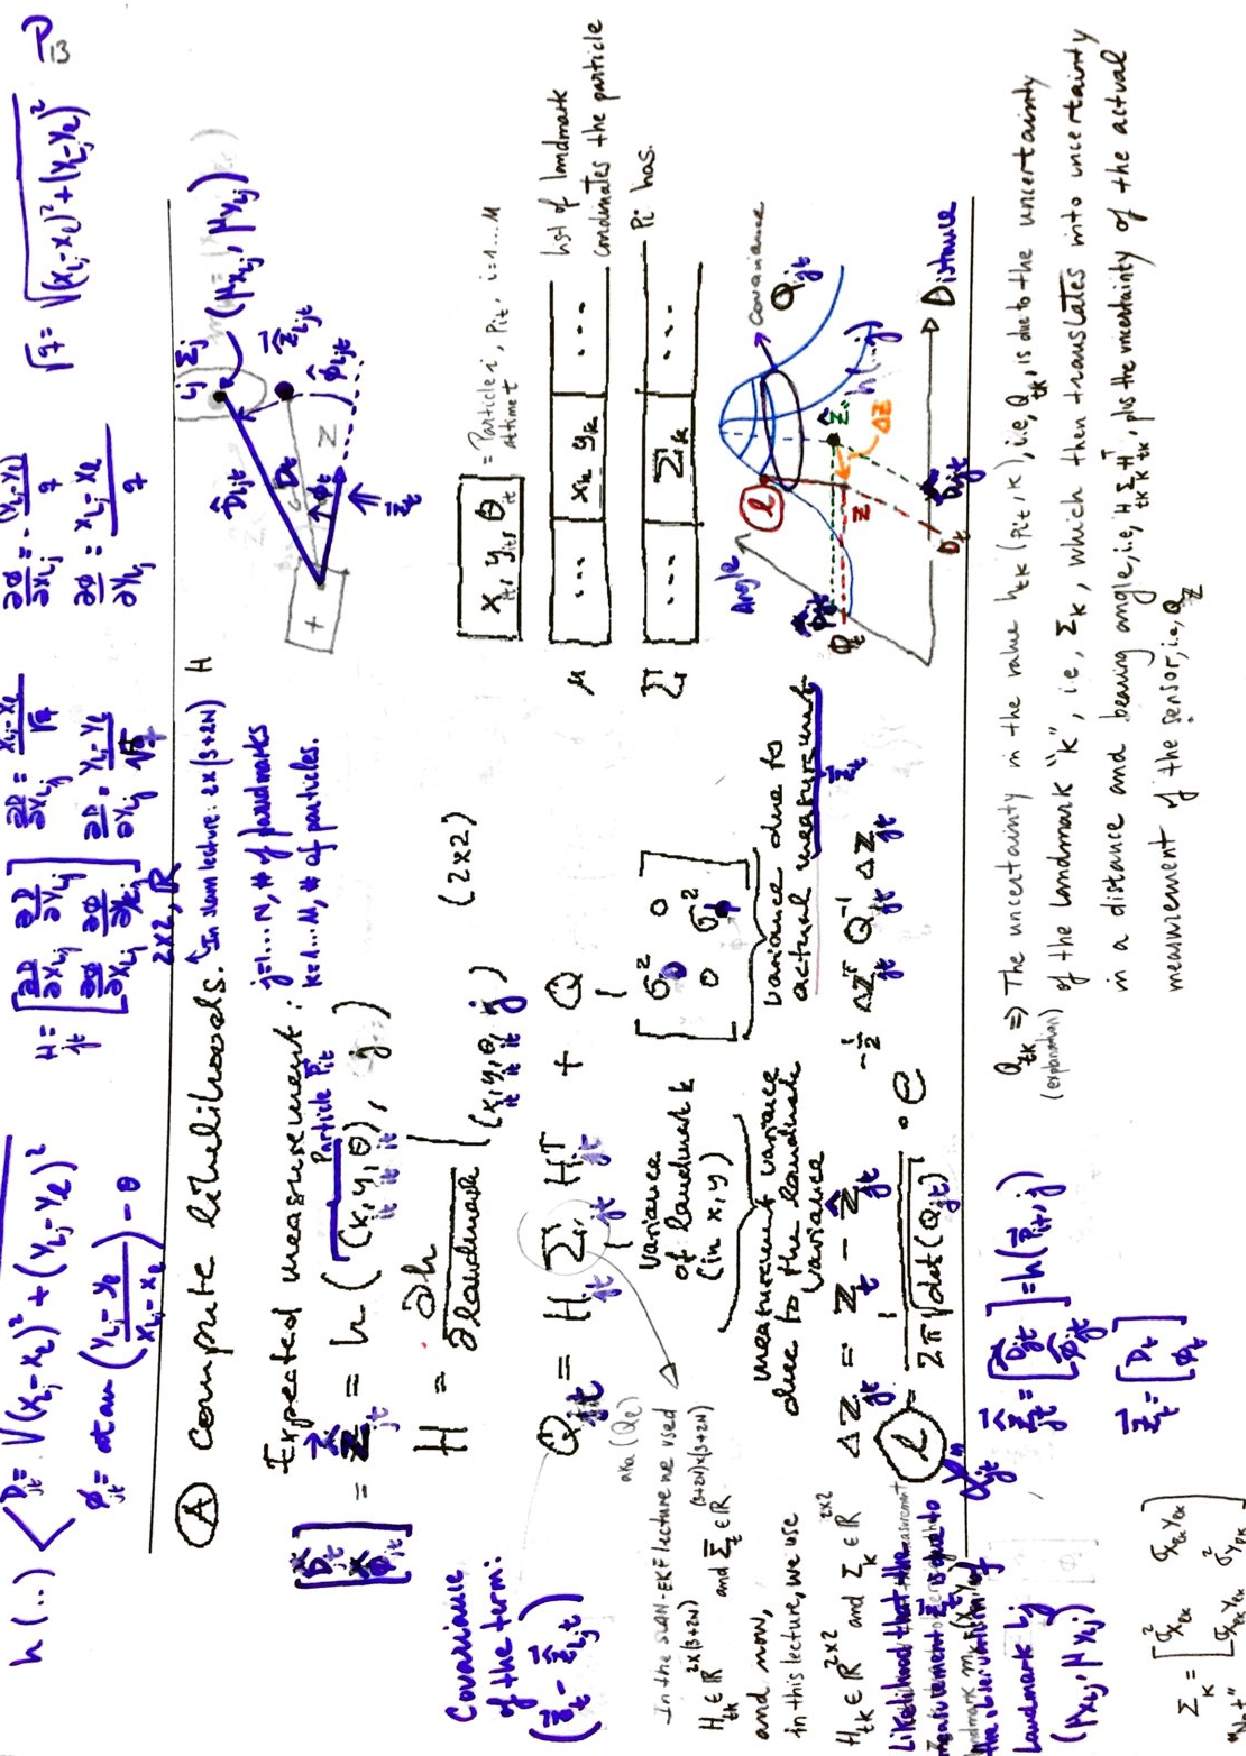
\includegraphics[clip,scale=0.75]{../FIGURES/fig43}
\end{figure}
 

\begin{figure}[H]
\centering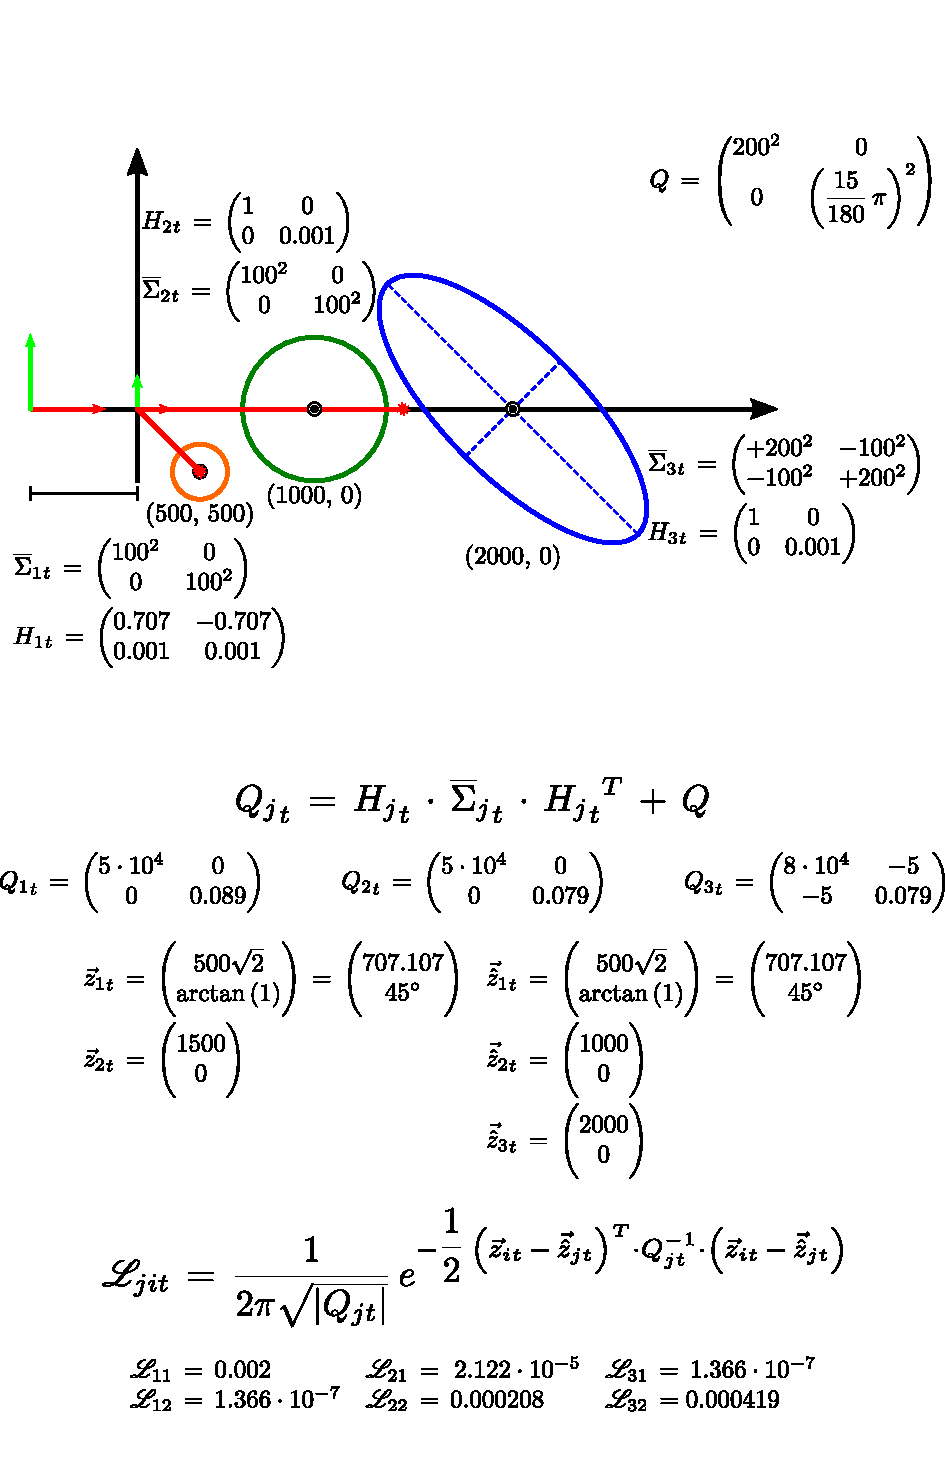
\includegraphics[clip,scale=0.9]{../FIGURES/fig49}
\end{figure}

\begin{figure}[H]
\centering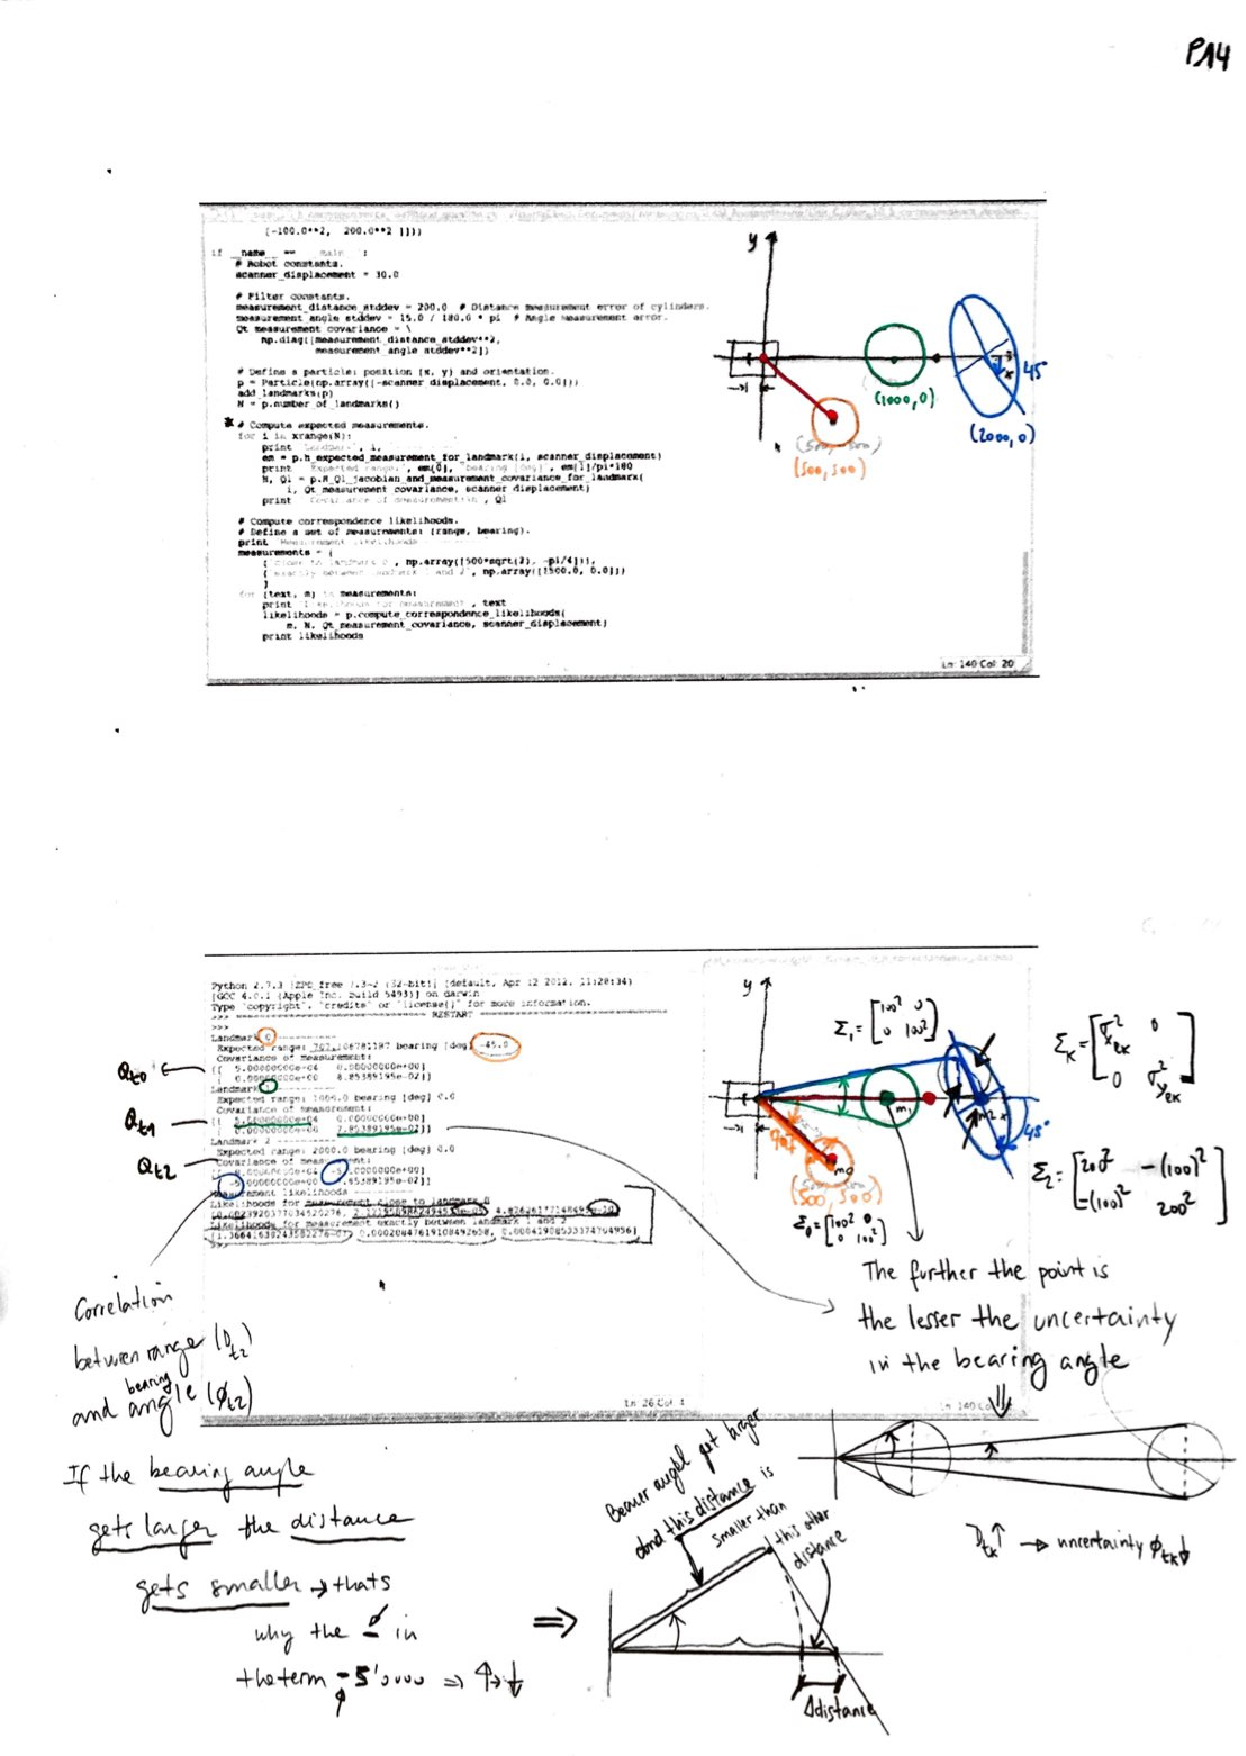
\includegraphics[clip,scale=0.85]{../FIGURES/fig47}
\end{figure}

\begin{figure}[H]
\centering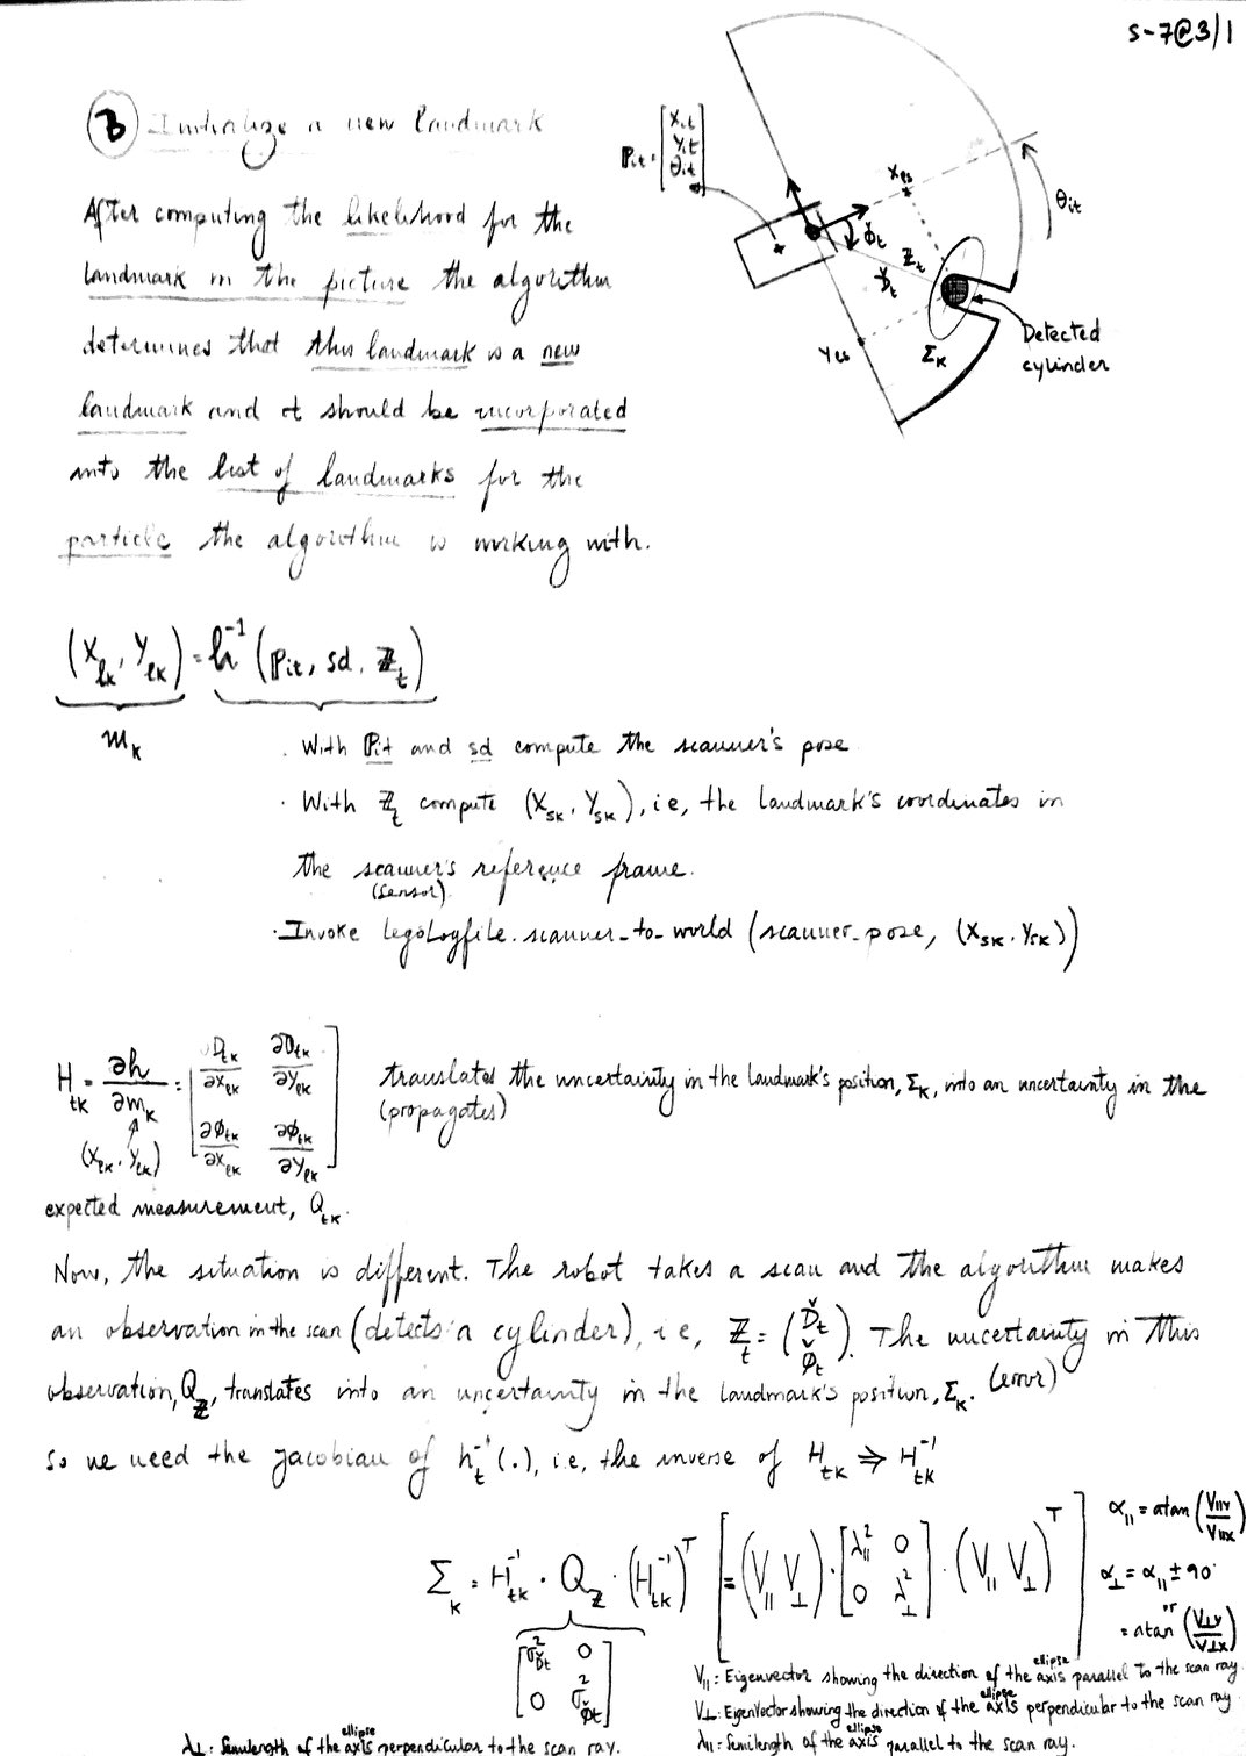
\includegraphics[clip,scale=0.85]{../FIGURES/fig50}
\end{figure}

\begin{figure}[H]
\centering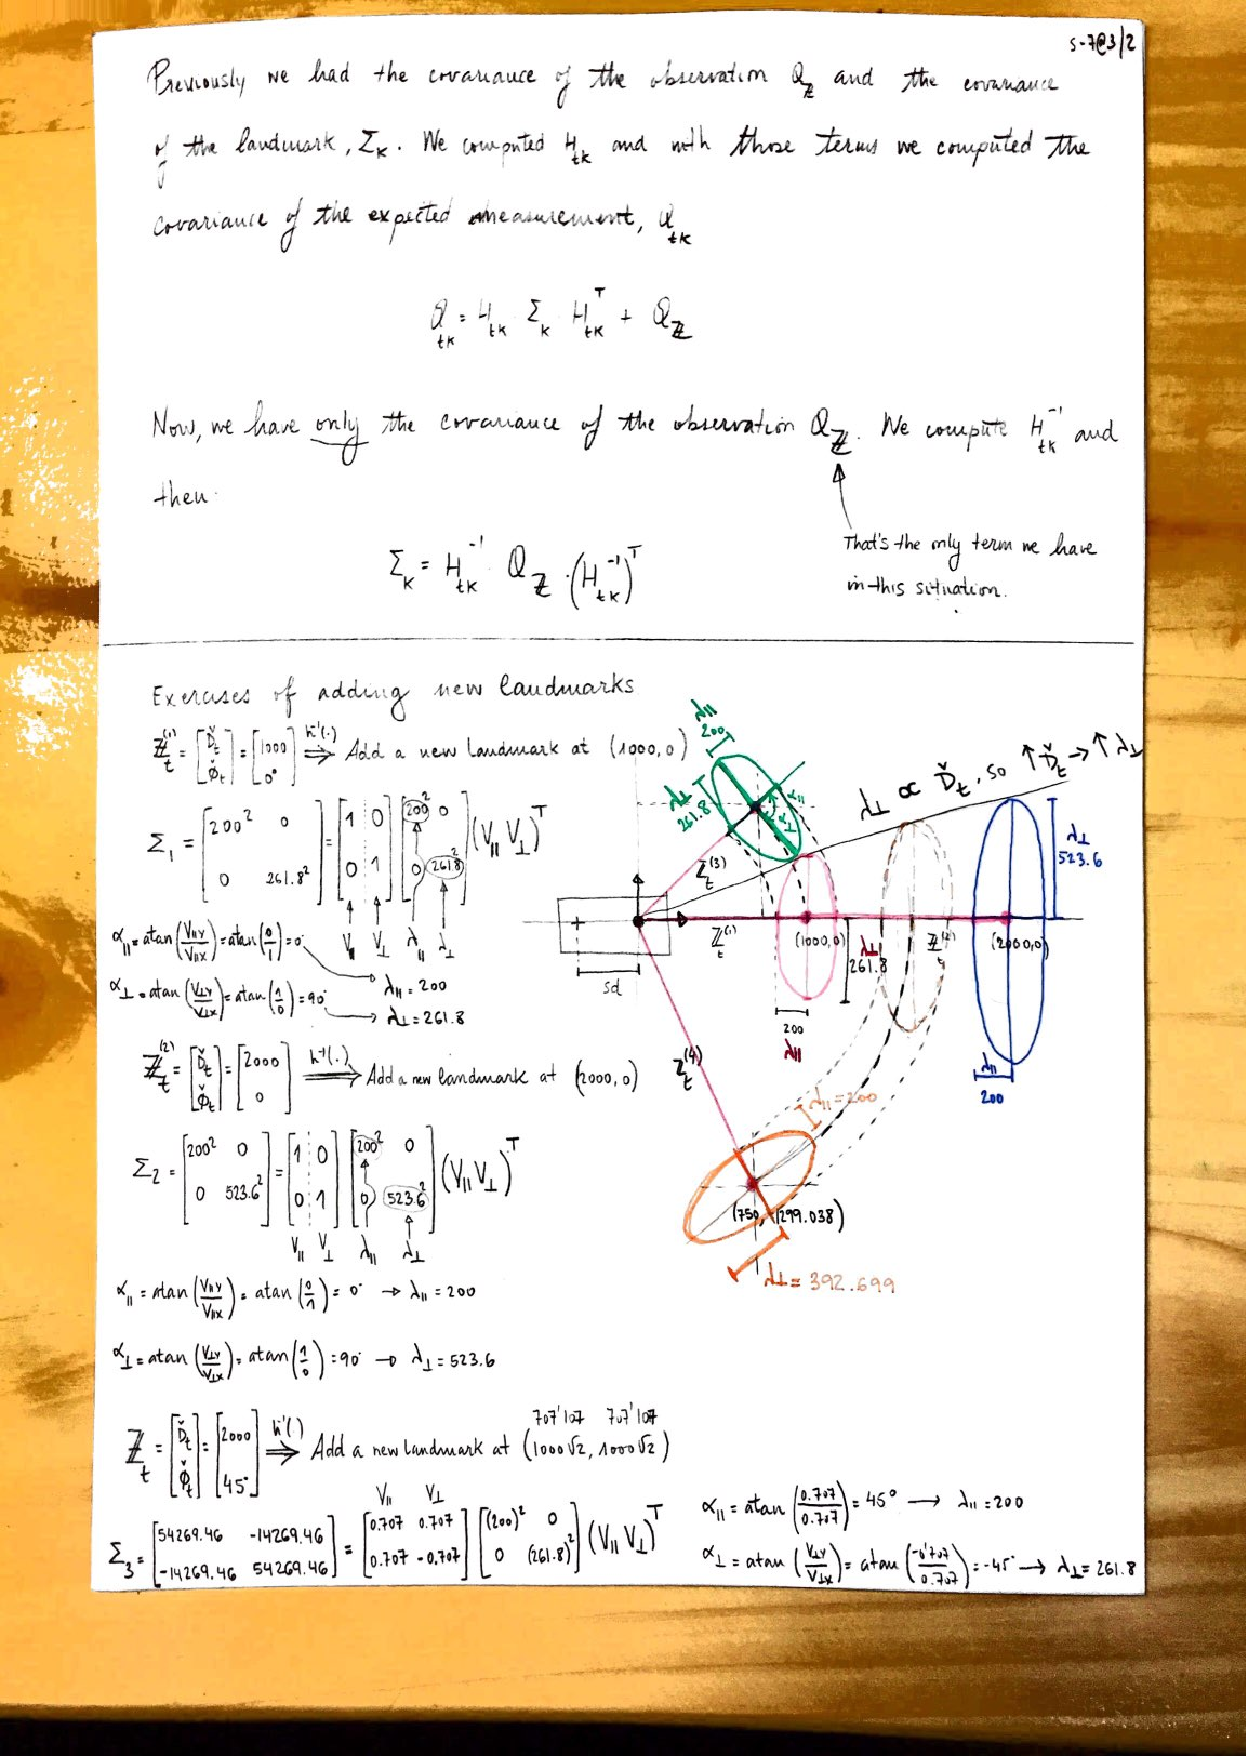
\includegraphics[clip,scale=0.85]{../FIGURES/fig51}
\end{figure}

\begin{figure}[H]
\centering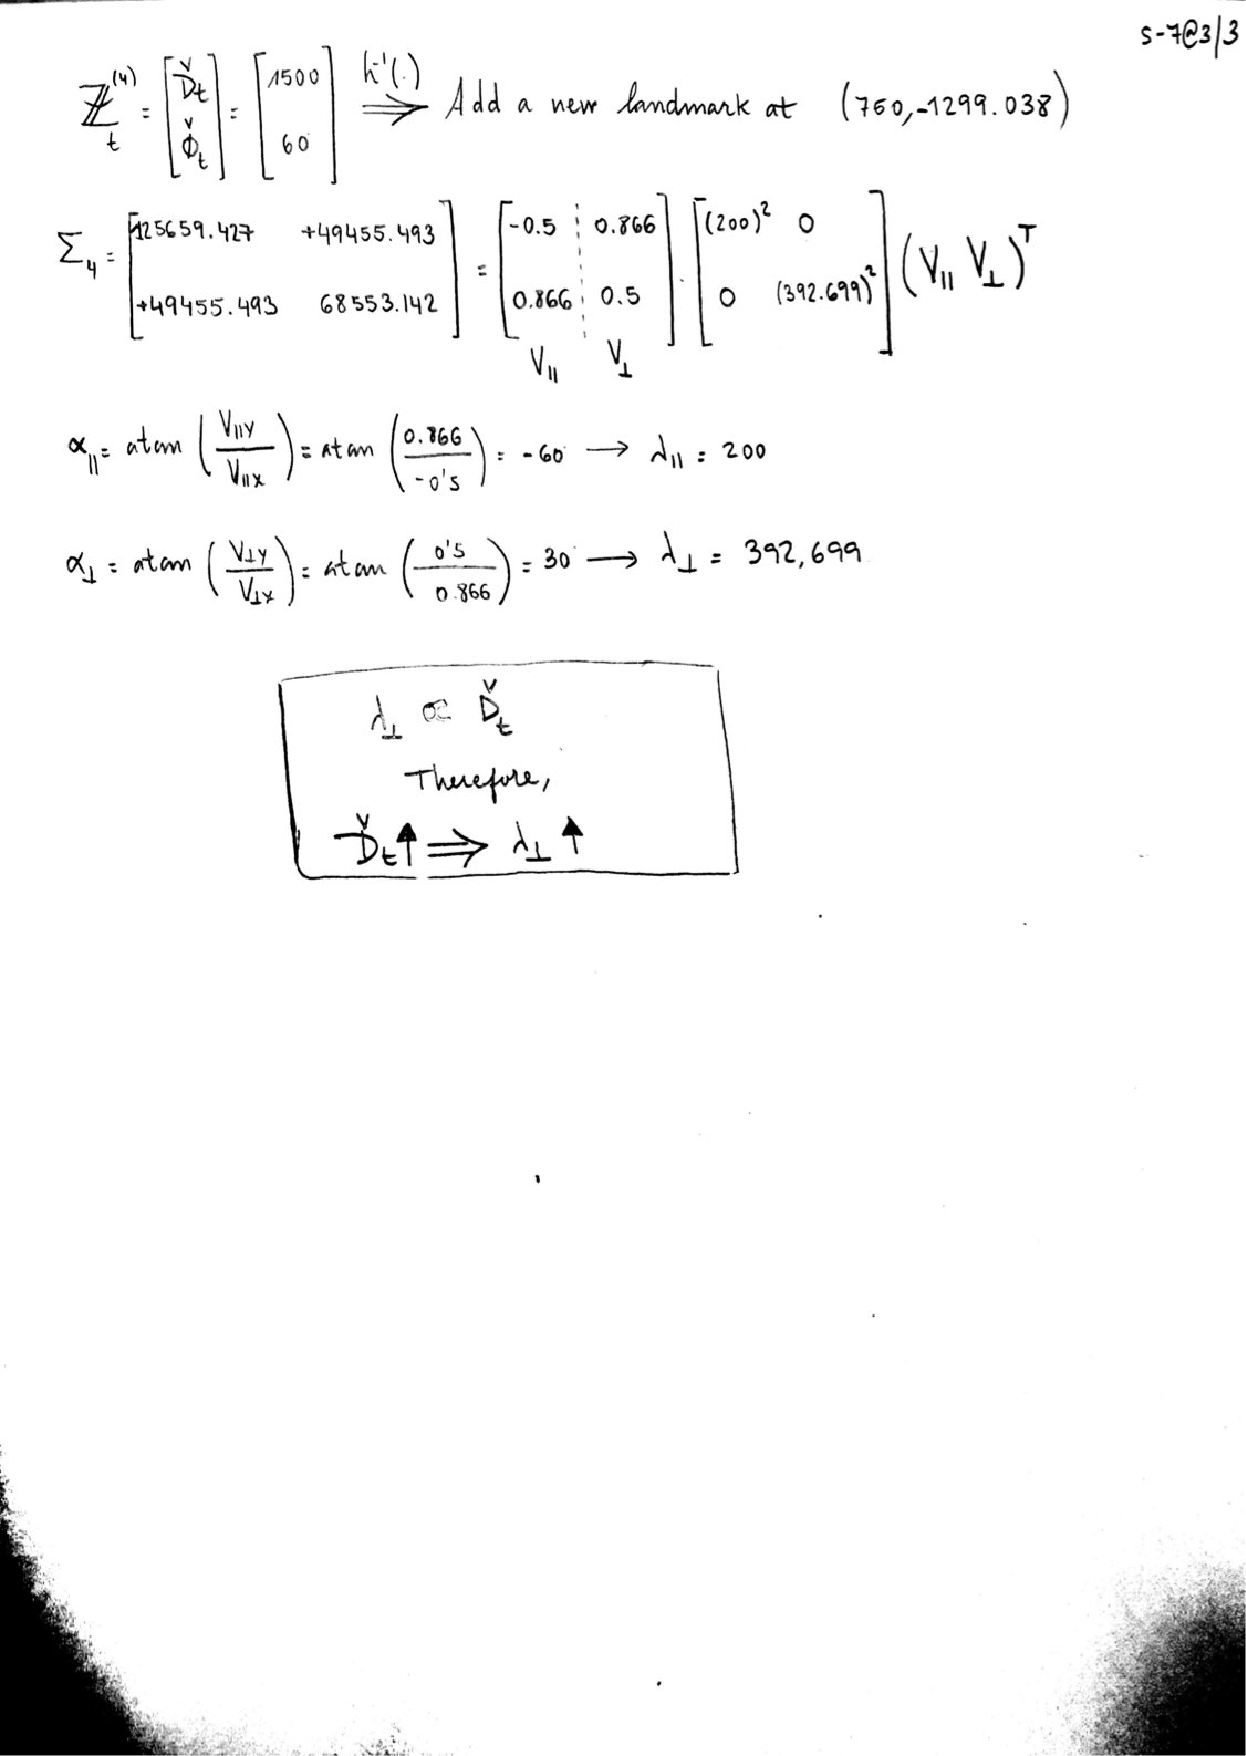
\includegraphics[clip,scale=0.85]{../FIGURES/fig52}
\end{figure}

\begin{figure}[H]
\centering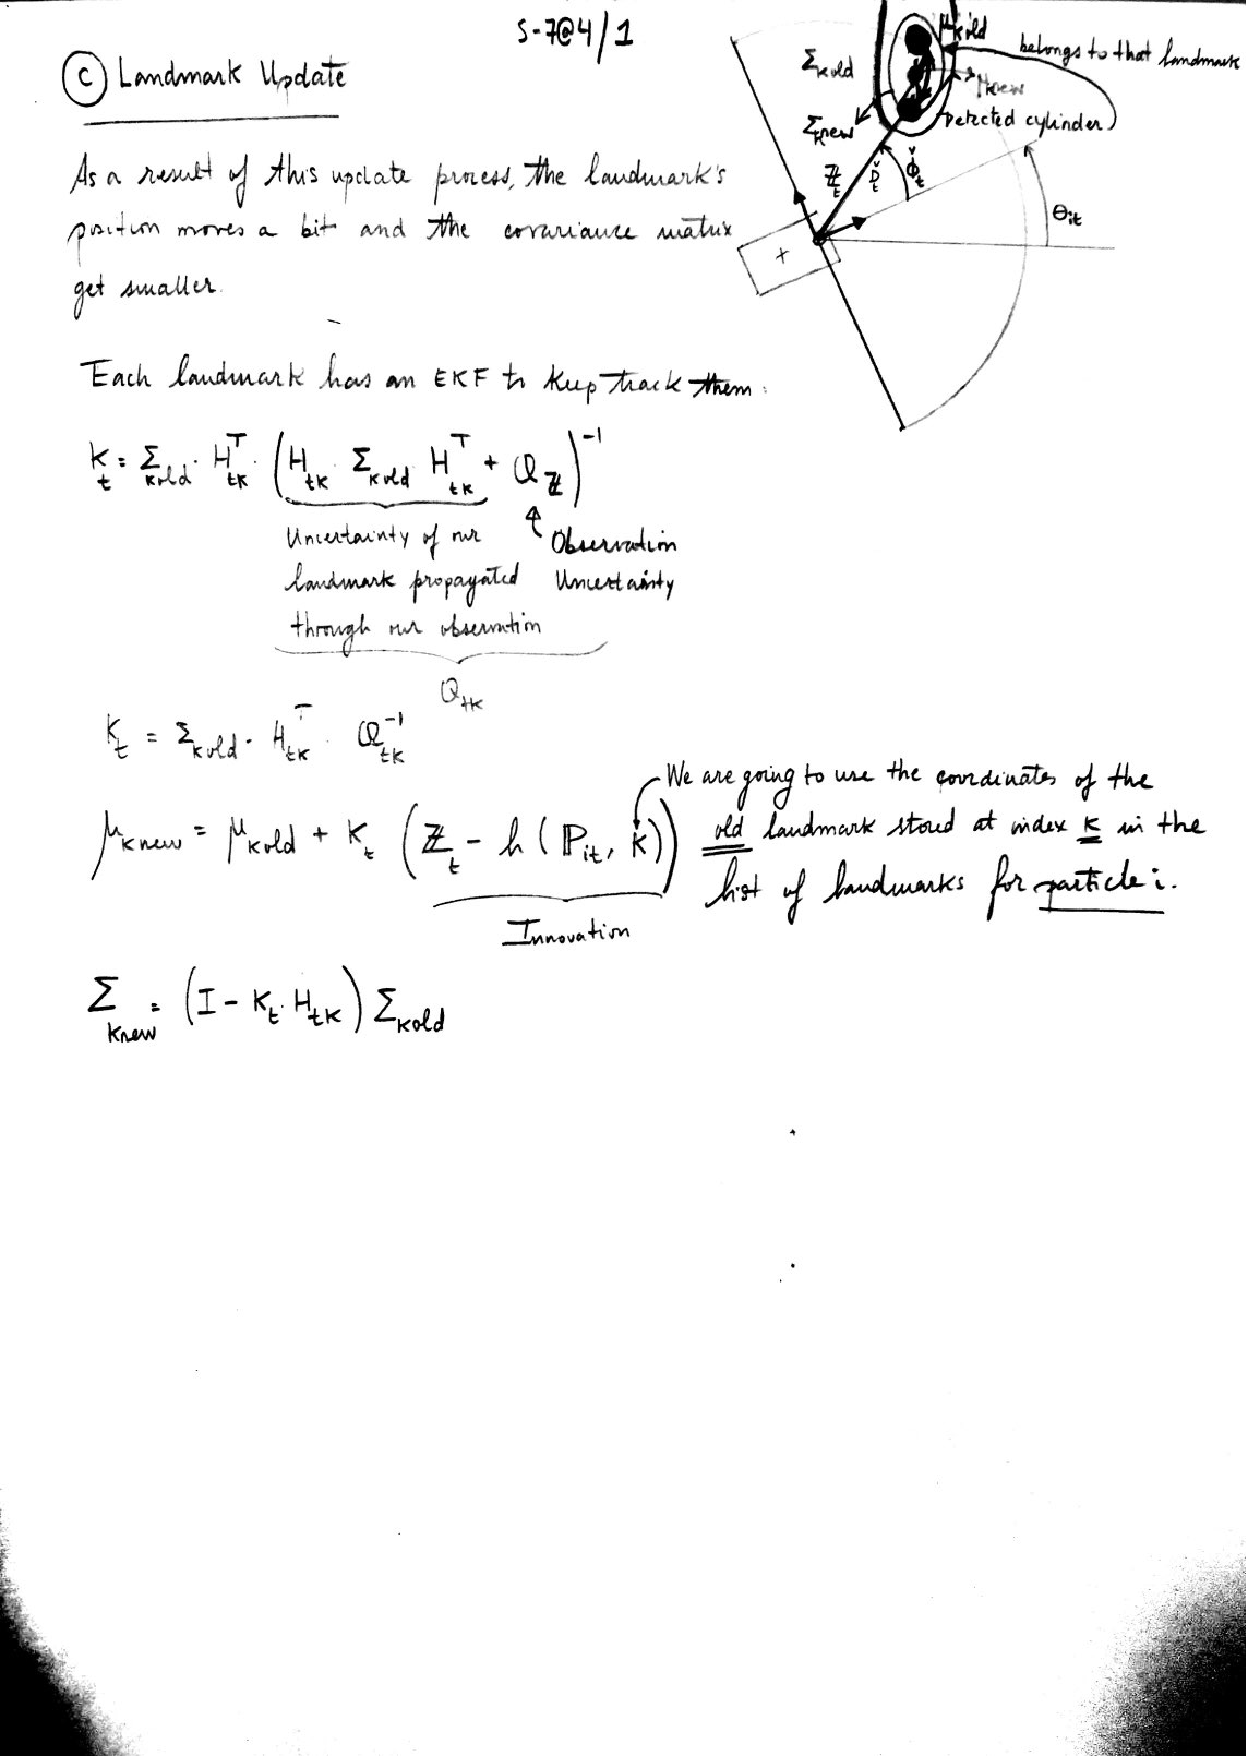
\includegraphics[clip,scale=0.85]{../FIGURES/fig53}
\end{figure}

\begin{figure}[H]
\centering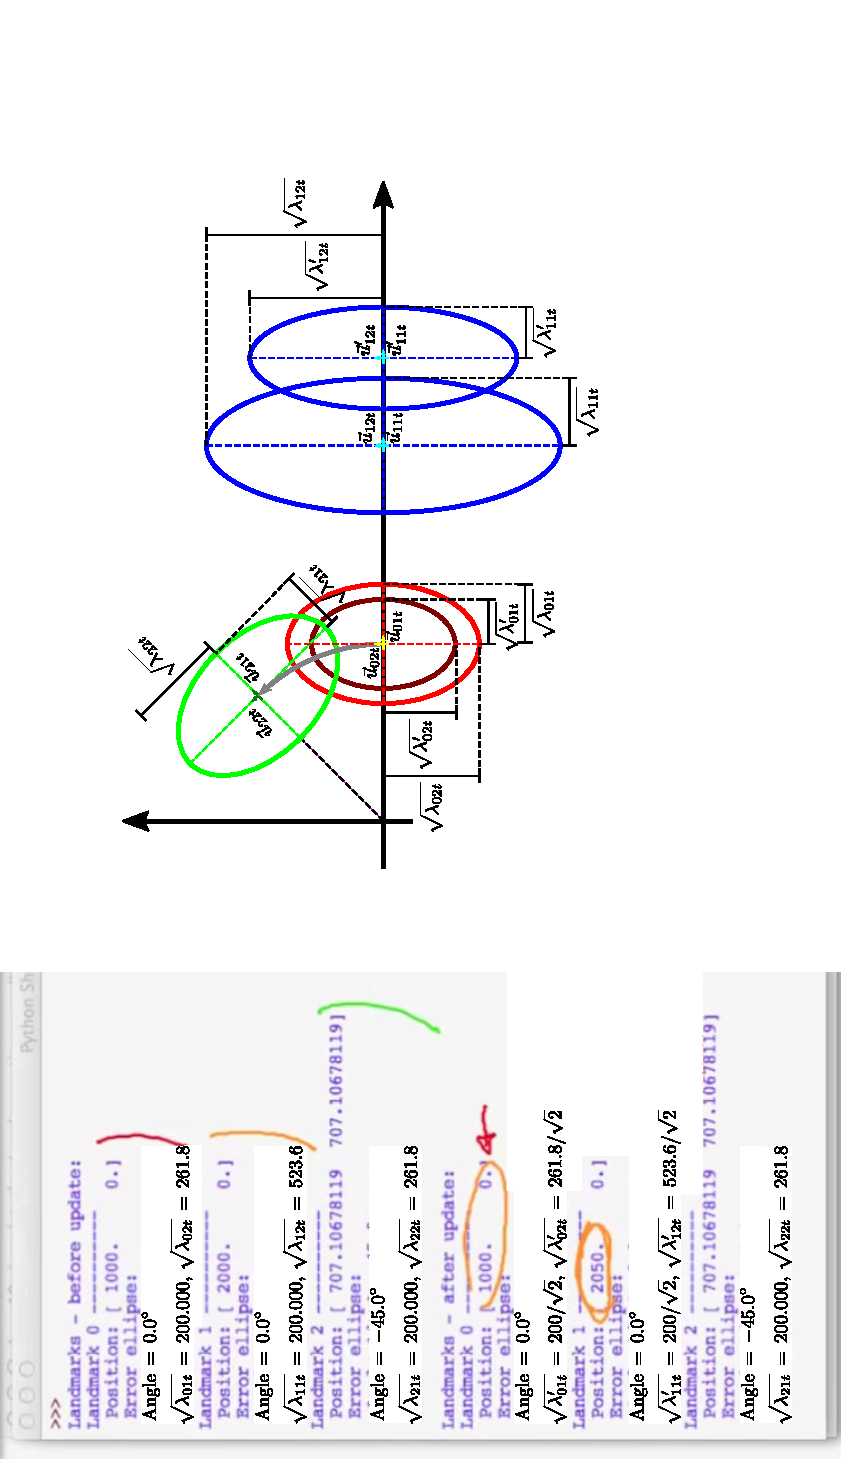
\includegraphics[clip,width=1\textwidth,height=1\textheight,keepaspectratio]{../FIGURES/fig57}
\end{figure}

\begin{figure}[H]
\centering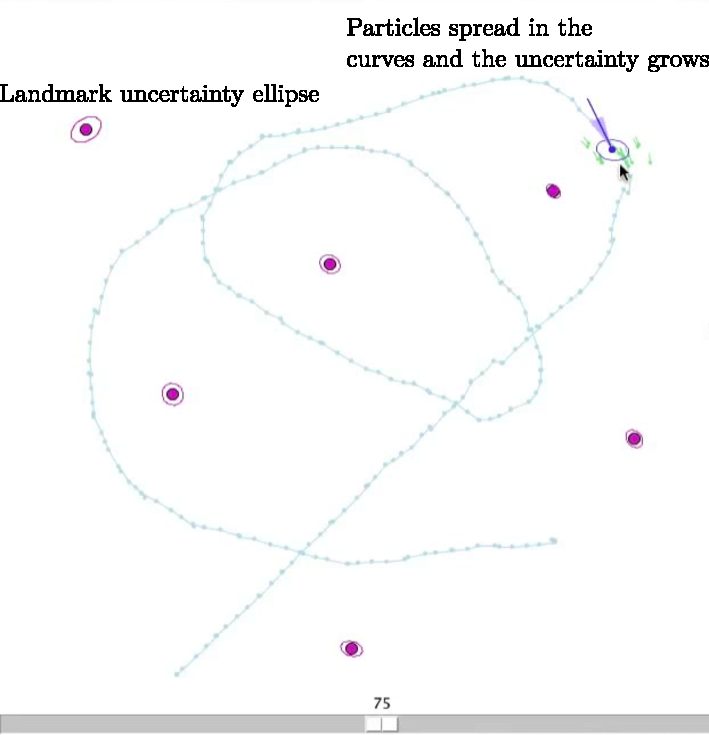
\includegraphics[clip,scale=0.82]{../FIGURES/fig59}
\end{figure}

\begin{figure}[H]
\centering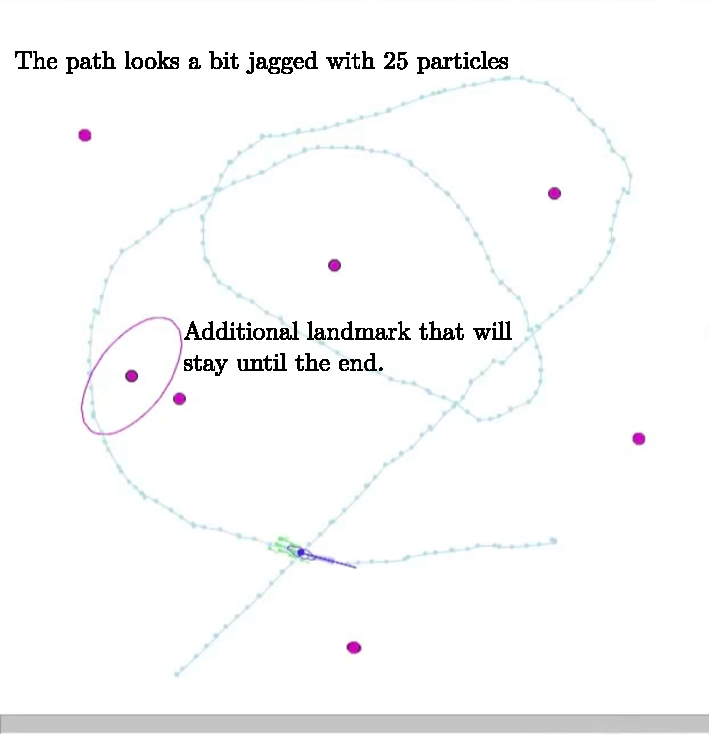
\includegraphics[clip,scale=0.82]{../FIGURES/fig61}
\end{figure}

That additional landmark appears in a particle at some point of the
execution of the algorithm and stays till the end of its execution.
This happens because the particle that contains the estimated position
and covariance matrix of that ellipse is duplicated during the resampling
process, probably because it's very close to the mean state. Posterior
resampling processes duplicate that landmark over and over again until
that landmark is presented in every particle. None of the measurements
taken by the laser scanner is assigned to that landmark anymore. Therefore,
it's necessary to find a way to get rid of those ghosts landmarks
that appear at some point in time.
\end{document}
